\makeatletter
\def\input@path{{../../}}
\makeatother
\documentclass[../../main.tex]{subfiles}
\graphicspath{
  {../../img/}
  {../img/}
  {img/}
}

\begin{document}
  
  \section{Множества и окрестности в $\R^n$}
  Далее в метрическом пространстве $(\R^n, \rho)$ для записи его 
  элементов (векторов) будем использовать не только малые буквы
  $a, b, c, \dots x$, но и большие $K, L, M, \dots$, а сами 
  элементы будем также называть точками.
  
  \emph{Открытым шаром} $B_r(x_0)$ радиуса $r > 0$ с центром в $x_0 \in 
  \R^n$ в пространстве ($\R^n, \rho$) будем называть множество 
  \[
  B_r(x_0) = \{x \in \R^n\ |\ \rho(x, x_0) < r\}, 
  \]
  А \emph{замкнутым шаром}
  \[
  \overline{B_r}(x_0) = \{x \in \R^n\ |\ \rho(x, x_0) \leqslant r\}, 
  \] 
  Очевидно, что $\overline{B_r}(x_0) = B_r(x_0) \cup S_r(x_0),$ где $ 
  S_r(x_0)$~--- $n$-мерная сфера в  $(\R^n, \rho)$, то есть 
  \[
  S_r(x_0) = \{x \in \R^n\ |\ \rho(x, x_0) = r\}
  \] 
  Шары $B_r, \overline{B_r}$ будем называть также \emph{открытыми} и 
  \emph{замкнутыми окрестностями} для $x_0 \in \R^n$. В случае, 
  когда размеры окрестностей не существенны или фиксированы, 
  будем их обозначать для краткости $V(x_0) = B_r(x_0)$ и 
  $\overline{V}(x_0) = \overline{B_r}(x_0)$.
  
  \smallskip
  \textbf{Примеры:}
  \begin{itemize}
  \item Для $n = 1 \implies d(x, x_0) = |x - x_0|, x, x_0 \in \R.
  $ В этом случае 
  \[
    B_r(x_0) = \{x \in \R\ |\ |x - x_0| < r\} =\ ] x_0 - r, x_0 + r [,
  \]
  \[
    \overline{B_r}(x_0) = \{x \in \R\ |\ |x - x_0| \leqslant r\} =\ 
    [ x_0 - r, x_0 + r ].
  \]
  Геометрически имеем:
  
  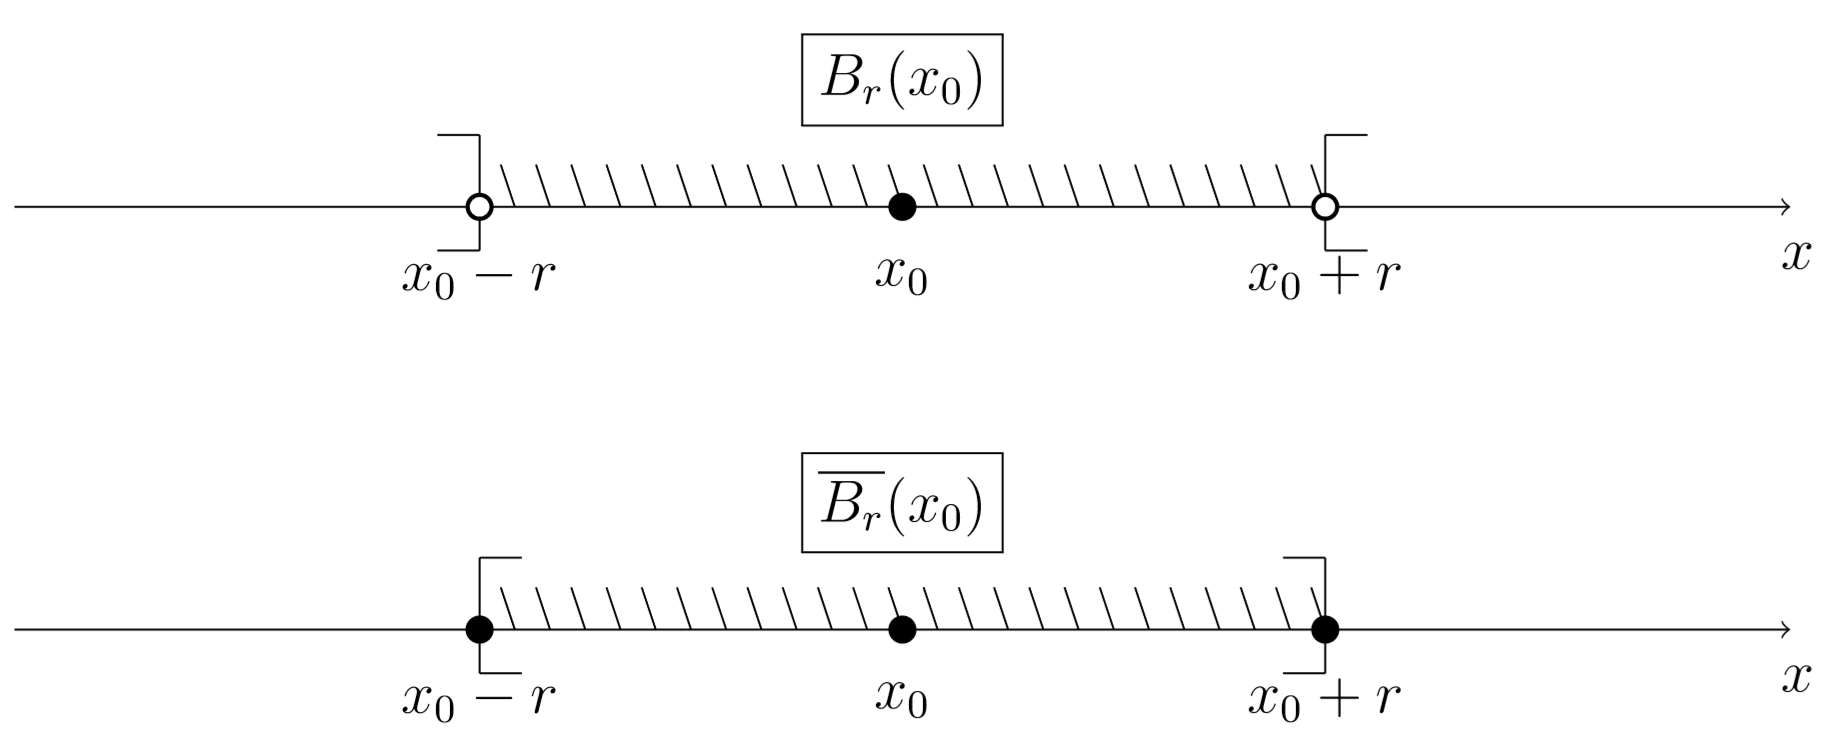
\includegraphics[width=\linewidth]{2019-02-15_17-21-02.png}
  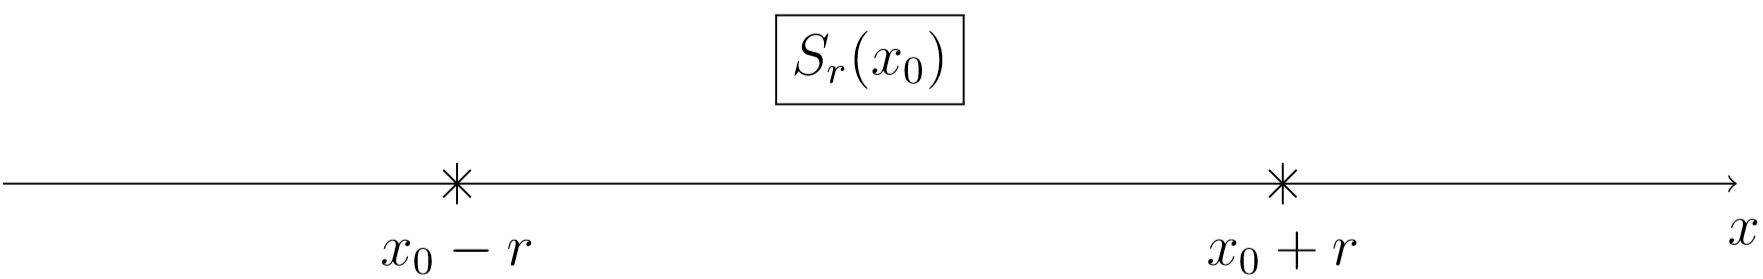
\includegraphics[width=\linewidth]{2019-02-15_17-21-17.png}
  
  \item  Для $M(x, y) \in \R^2$ в ДПСК имеем для $M_0(x_0, y_0)$:
  \[
    d(M, M_0) = \sqrt{(x - x_0)^2 + (y - y_0)^2}.
  \]
  Поэтому открытым шаром от $M_0$ здесь будет открытый круг 
  \[
    (x - x_0)^2 + (y - y_0)^2 < r^2,
  \]
  а замкнутым шаром будет замкнутый круг 
  \[
    (x - x_0)^2 + (y - y_0)^2 \leqslant r^2,
  \]
  а сфера является окружностью 
  \[
    (x - x_0)^2 + (y - y_0)^2 = r^2.
  \]
  
  \item Аналогично для $n = 3$ для $M_0(a, b, c) \in \R^3$ и $M(x, 
  y, z) \in \R^3$ в соответствующей ДПСК имеем  
  \[
    d(M, M_0) = \sqrt{(x - x_0)^2 + (y - y_0)^2 + (z - z_0)^2}.
  \]
  Поэтому:
  
  $B_r$~--- это открытый шар
  \[
    (x - x_0)^2 + (y - y_0)^2 + (z - z_0)^2 < r,
  \]
  $\overline{B_r}$~--- это замкнутый шар
  \[
  (x - x_0)^2 + (y - y_0)^2 + (z - z_0)^2 \leqslant r,
  \]  
  $S_r$~--- трехмерная сфера
  \[
  (x - x_0)^2 + (y - y_0)^2 + (z - z_0)^2 = r.
  \]
  \end{itemize}
  \begin{exc}
    Для $n = 1, 2, 3$  выяснить геометрический смысл $B_r(M_0), 
    \overline{B_r}(M_0),  S_r(M_0)$ в пространствах $(\R^n, \rho_1)$ 
    и $(\R^n, \rho_2)$  с соответствующими октаэдрической метрикой 
    $\rho_1$ и кубической метрикой $\rho_2$. 
  \end{exc}
  \begin{rem}
    Кроме полных окрестностей $B_r(x_0), \overline{B_r}(x_0)$ в $
    (\R^n, \rho)$ будем рассматривать выколотые окрестности в $
    (\R^n, \rho)$ то есть множества
    \[
      \dot{B_r}(M_0) = B_r(M_0) \backslash \{M_0\},
    \]
    \[
      \dot{\overline{M_r}}(M_0) = \overline{B_r}(M_0) \backslash \{M_0\},
    \]
    которые для краткости иногда будем обозначать $\dot{V}(M_0) $ и 
    $\dot{\overline{V}}(M_0)$ соответственно. 
  \end{rem}
  \smallskip
  
  Точку $M_0 \in D,$ где $D \subseteq \R^n$, будем называть 
  \emph{изолированной} для множества $D$, если $\exists V(M_0) \subset 
  \R^n$ в которой нет других точек из $D$, кроме $M_0$.
  
  Точку $M_0 \in \R^n$ будем называть \emph{граничной} для $D \subset \R^n,
  $ если в любой окрестности $V(M_0) \subset \R^n$ есть точки как 
  принадлежащие $D$, так и не входящие в $D$.
  
  Точку $M_0 \in D$ будем называть \emph{внутренней} для $D \subset \R^n$, 
  если $\exists V(M_0) \subset D$.
  
  Точку $M_0 \in D$ будем называть \emph{предельной} для $D \subset \R^n$, 
  если $\forall V(M_0) \subset \R^n$ есть точки как входящие, так и 
  не входящие в $D$.
  Можно показать, что $M_0 \in \R^n$ будет предельной для $D \subset 
  \R^n$ тогда и только тогда, когда $M_0$ либо внутренняя для $D$, 
  либо граничная.
  Очевидно, что любая изолированная точка не является предельной для 
  $D$.
  
  Для $D \subset \R^n$ множество его граничных точек называют 
  \emph{границей множества} и обозначают $\partial D$. 
  $\forall D \subset \R^n$ множество $\overline D = D \cup \partial D$ 
  называется \emph{замыканием множества} $D$. 
  Множество $D \subset \R^n$ считают \emph{замкнутым} в $\R^n$, если  $D = \overline 
  D$.
  
  Множество $D \subset \R^n$ называют \emph{открытым} в $\R^n$, если любая 
  его точка является внутренней для $D$. Нетрудно видеть, что 
  множество $D \subset \R^n$ будет открытым тогда и только тогда, 
  когда его дополнение $\R^n \backslash D$ замкнуто в $\R^n$. 
  
  \smallskip
  Открытые множества в $\R^n$ обладают следующими основными 
  свойствами:
  \begin{enumerate}
    \item
     $\R^n$  и $\varnothing$ являются открытыми в $\R^n$; 
     \item
      Объединение \emph{любого} числа открытых множеств в $\R^n$~--- 
      открытое множество в $\R^n$; 
      \item Пересечение \emph{конечного} числа открытых множеств в 
      $\R^n$ является открытым множеством в $\R^n$.
  \end{enumerate}  

  Аналогичными свойствами обладают замкнутые множества в $\R^n$:
  \begin{enumerate}
    \item  $\R^n$  и $\varnothing$ замкнуты в $\R^n$;
    \item Объединение \emph{конечного}  числа замкнутых множеств в 
    $\R^n$ является замкнутым множеством в $\R^n$; 
    \item Пересечение \emph{любого} числа замкнутых множеств в $\R^n$ 
    является замкнутым множеством в $\R^n$.
  \end{enumerate} 
  
  
  В дальнейшем множество $D \subset \R^n$ будем называть 
  \emph{ограниченным} в линейном метрическом пространстве $ (\R^n, \rho) $, 
  если все точки из $D$ расположены внутри некоторого $n$-мерного шара 
  конечного радиуса.
  
  \begin{exc}
    Показать, что на множестве действительных чисел функция 
    \[ 
      \rho(x, y) = \frac{|x - y|}{1 + |x - y|}
    \] удовлетворяет всем аксиомам расстояния, и при этом в 
    получаемом метрическом пространстве $ (R, \rho) $ все множества 
    (даже бесконечные промежутки) будут ограниченными.   
   \end{exc} 
 
  \smallskip   
  В общем случае, любое ограниченное замкнутое множество $D \subset 
  \R^n$ метрического пространства $ (\R^n, \rho) $ называется 
  \emph{компактом} в $\R^n$.
  Множество $D \subset \R^n$ считается \emph{связным}, если любые две точки 
  $M1,M2 \in D $ можно соединить некоторой непрерывной линией $ l = 
  \widehat{M_1M_2} \subset D$  
  т.е. имеющей параметризацию
  \[
    l = \{x = x(t) \in D\ |\ x(t) = (x_1(t), \dots, x_n(t))\},
  \]
  где $\forall x_k(t)$~--- непрерывная функция от $t \in [\alpha, 
  \beta], k = \overline{1,n},$ причем $ x(\alpha) = M_1, x(\beta) = 
  M_2.$
   
  Открытое связное множество $D \subset \R^n$ в метрическом 
  пространстве $ (\R^n, \rho) $ называют \emph{областью} в $\R^n$, а 
  его замыкание $D$ называют \emph{замкнутой областью} в $\R^n$.
   
  Далее, как правило, будем использовать открытые связные множества 
  из $\R^n$.
  
\end{document}
